\documentclass[12pt, oneside]{article}
\usepackage[letterpaper, margin=1in, headsep=0.5in]{geometry}
\usepackage[english]{babel}
\usepackage[utf8]{inputenc}
\usepackage{amsmath}
\usepackage{amsfonts}
\usepackage{amssymb}
\usepackage{tikz}
\usetikzlibrary{quotes, angles}
\usepackage{graphicx}
%\usepackage{pgfplots}
%\pgfplotsset{width=10cm,compat=1.9}
%\usepgfplotslibrary{statistics}
%\usepackage{pgfplotstable}
%\usepackage{tkz-fct}
%\usepackage{venndiagram}

\usepackage{fancyhdr}
\pagestyle{fancy}
\fancyhf{}
\rhead{\thepage \\Name: \hspace{1.5in}.\\}
\lhead{BECA / Dr. Huson / 11.1 IB Math\\* Unit 1: Algebra Review}

\renewcommand{\headrulewidth}{0pt}

\begin{document}

\subsubsection*{1-3 Homework: Function substitution}
Answer on loose leaf paper in pen, or, for the graphs, on graph paper in pencil. Show working for all problems.

\begin{enumerate}

\item For the function $f(x) = 2x-7$
\begin{itemize}
  \item[(a)] What is the value of $f(3)$?
	\item[(b)] Solve for $x$ if $f(x)=0$.
	\item[(c)] Find  $f(1-x)$.
	\item[(d)] Solve for $x$ if $f(x)=x$.
\end{itemize}

\item For the function $g(x) = x^2-4$ with $x>0$
\begin{itemize}
  \item[(a)] Simplify the expression $g(x-3)$
	\item[(b)] Solve $g(x)=0$.
  \item[(c)] Write down the domain and range of the function $g$.
\end{itemize}

\item For the functions $f(x) = 2-x^2$ and $g(x) = 2x+3$
\begin{itemize}
  \item[(a)] What is the value of $g(3)$?
	\item[(b)] Solve $f(x)=g(x)$.
\end{itemize}

\item Given that $g(x) = \frac {1}{3} x+3$
\begin{itemize}
  \item[(a)] Find $g(\frac{9}{2})$.
	\item[(b)] At what point does the graph of $g(x)$ cross the $y$-axis?
\end{itemize}

\item For the functions defined by $f(x) = 2x$ and $g(x) = x+4$
\begin{itemize}
  \item[(a)] Find an expression for $(f+g)(x)=f(x)+g(x)$.
	\item[(b)] Find $(f+g)(-4)$.
\end{itemize}

\item Write down the domain and range of $f(x)= x^2-6$. Use set notation (i.e. brackets)

\item Using a GDC to analyze the function $\displaystyle f(x)= \frac {3x+2}{x+1}$
\begin{itemize}
    \item[(a)] Write down the equations for the asymptotes.
	\item[(b)] Write down the domain and range of $f(x)$.
\end{itemize}

\newpage

\item Write down the domain and range of the function graphed using set notation.

\begin{figure}[!ht]
    \centering
    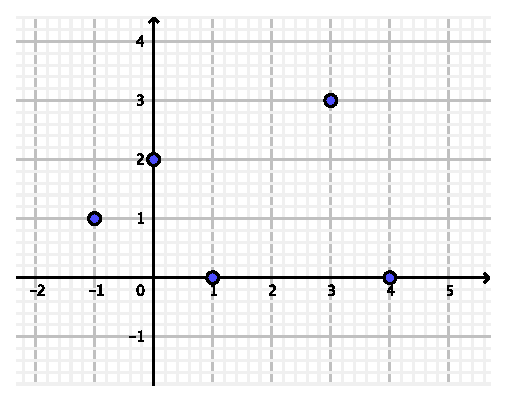
\includegraphics[width=0.5\textwidth]{1-4_domain.eps}
    %\caption{Write down domain and range. \label{domain}}
\end{figure}

\item For the function shown
\begin{figure}[!hb]
    \centering
    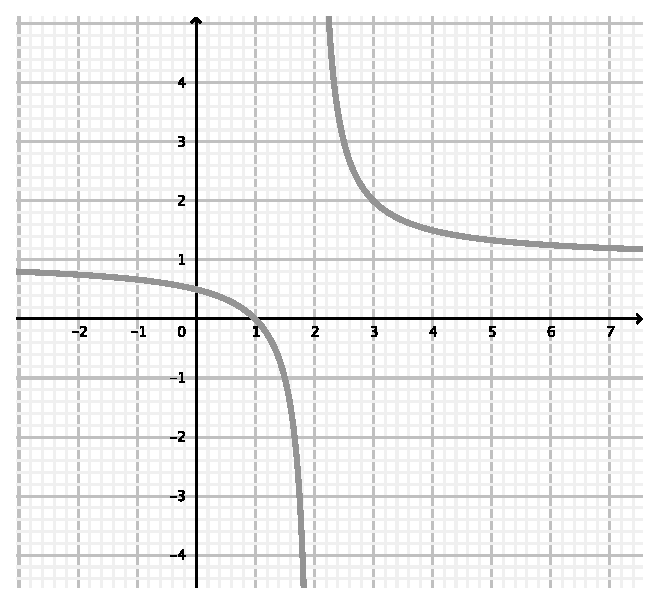
\includegraphics[width=0.5\textwidth]{1-4_asymptotes.eps}
    %\caption{Determine asymptotes. \label{asymptote}}
\end{figure}
\begin{itemize}
    \item[(a)] Write down the equations for the asymptotes.
	\item[(b)] Write down the domain and range of the function. Assume that the curves extend indefinitely horizontally and vertically.
\end{itemize}

\item Consider the function $f(x) = x^3 - 4x^2 - 3x + 18$.
\begin{itemize}
    \item[(a)] Find the values of $f(x)$ for $a$ and $b$ in the table below:\\
	\begin{tabular}{|l|c|c|c|c|c|c|c|c|c|}
	\hline
	$x$ & -3 & -2 & -1 & 0 & 1 & 2 & 3 & 4 & 5\\
	\hline
    $f(x)$ & -36 & $a$ & 16 & $b$ & 12 & 4 & 0 & 6 & 28\\
	\hline
	\end{tabular}
	%\item[(b)] Using a scale of 1 cm for each unit on the $x$-axis and 1 cm for each 5 units on the $y$-axis, draw the graph of $f(x)$ for $-3 \leq x \leq 5$. Label it clearly using IB conventions on the graph paper provided (other side).


\end{itemize}
\end{enumerate}

%missing: identifying a function vs relation,

\end{document}
